\documentclass[10pt, compress]{beamer}

\usetheme{m}

\usepackage{booktabs}
\usepackage[scale=2]{ccicons}
\usepackage{minted}
\usepackage{hyperref}
\usepackage{xcolor}

\usemintedstyle{trac}

\title{A few notes on workflow v2.0.0}
\subtitle{}
\date{\today}
\author{Mohammad-Ali \textsc{A'r\^abi} \& Karsten \textsc{Fix}}
\institute{AppTec Services GmbH}

\begin{document}

\maketitle

\section{Branch Naming}

\begin{frame}[fragile]
  \frametitle{Bad Practice}
  
  The following is not a good branch name:
  \begin{minted}[fontsize=\small]{bash}
bugfixes
  \end{minted}
  
  \begin{itemize}
      \item It's \textbf{not} descriptive.
      \item It does \textbf{not} mention the main maintainer of the branch.
      \item It does \textbf{not} mention the problem it's trying to solve.
  \end{itemize}

\end{frame}

\begin{frame}[fragile]
  \frametitle{Good Practice}
  
  The following branch name is good:
  \begin{minted}[fontsize=\small]{bash}
mar/fix-router-subscription-bug
  \end{minted}
  
  \begin{itemize}
      \item It is descriptive.
      \item It does mention the main maintainer of the branch.
      \item It does mention the problem it's trying to solve.
  \end{itemize}

\end{frame}

\begin{frame}[fragile]
  \frametitle{Better Practice}
  
  The following branch name is even better:
  \begin{minted}[fontsize=\small]{bash}
mar/18-fix-router-subscription-bug
  \end{minted}
  
  The number \texttt{18} refers to GitLab's ticket number.
  
  \begin{itemize}
      \item It is descriptive.
      \item It does mention the main maintainer of the branch.
      \item It contains a link the problem it's trying to solve.
  \end{itemize}

\end{frame}

\begin{frame}[fragile]
  \frametitle{GitLab Branch Creation}
  
  \begin{figure}
      \centering
      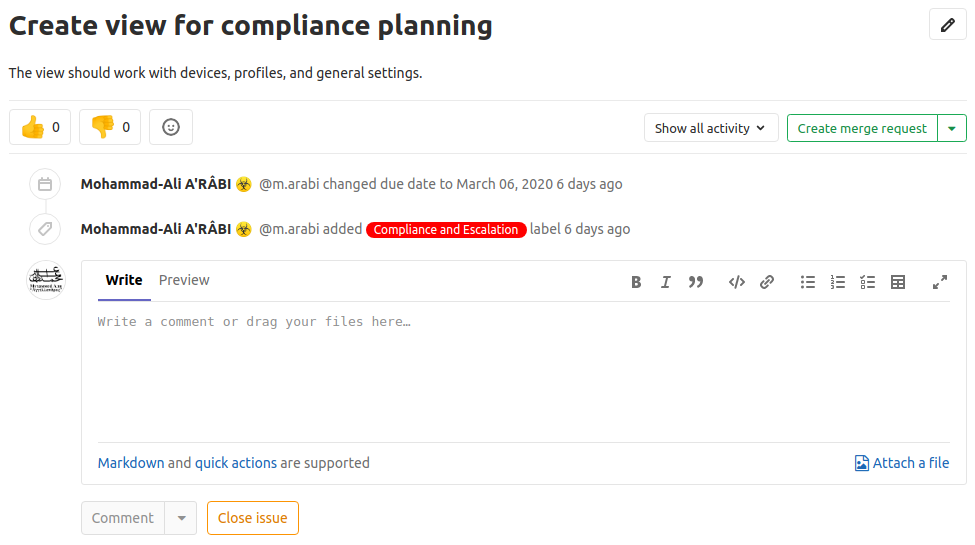
\includegraphics[scale=0.3]{images/gitlab-branch-1.png}
      \caption{GitLab issue view}
      \label{fig:gitlab1}
  \end{figure}

\end{frame}

\begin{frame}[fragile]
  \frametitle{GitLab Branch Creation}
  
  \begin{figure}
      \centering
      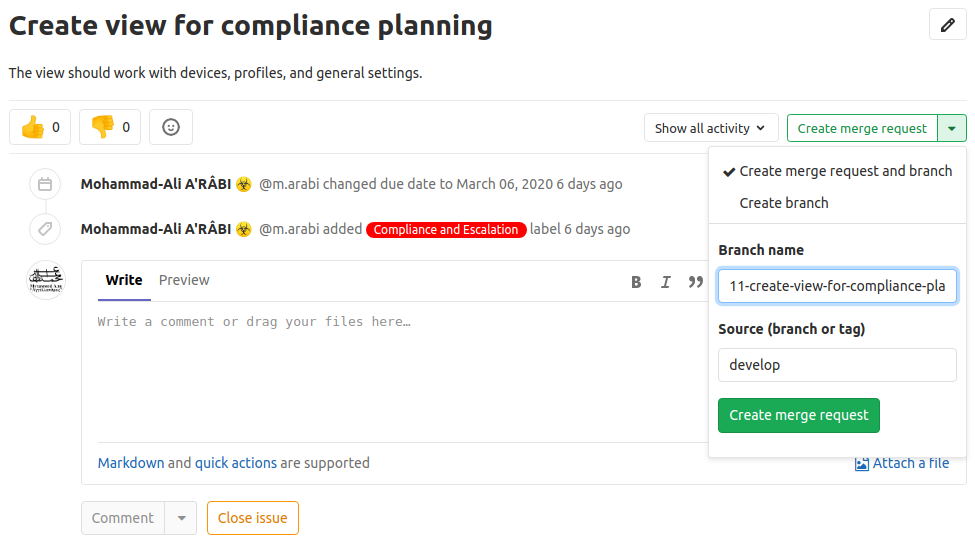
\includegraphics[scale=0.3]{images/gitlab-branch-2.png}
      \caption{GitLab issue view}
      \label{fig:gitlab2}
  \end{figure}

\end{frame}

\begin{frame}[fragile]
  \frametitle{GitLab Branch Creation}
  
  \begin{figure}
      \centering
      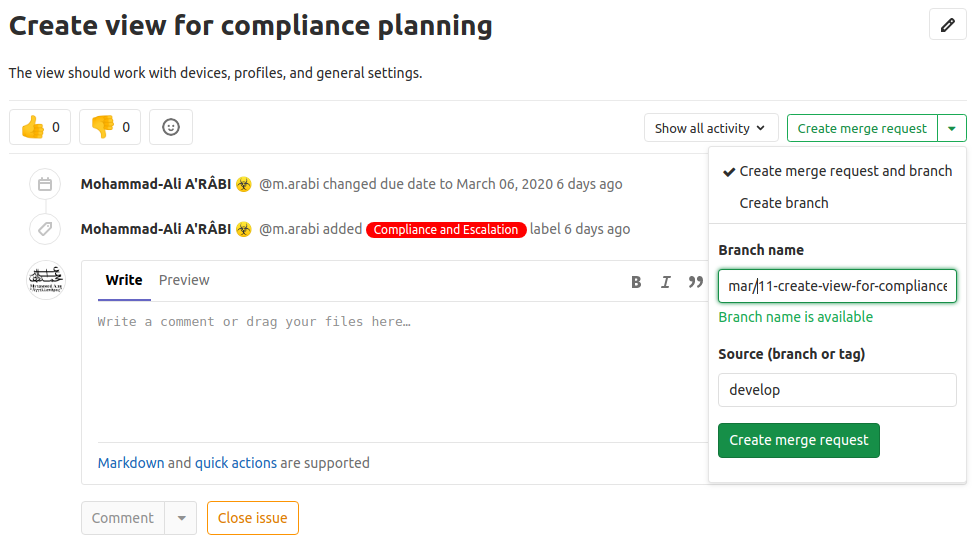
\includegraphics[scale=0.3]{images/gitlab-branch-3.png}
      \caption{GitLab issue view}
      \label{fig:gitlab3}
  \end{figure}

\end{frame}

\section{Commit Messages}

\begin{frame}[fragile]
  \frametitle{Bad Practice}
  
  The following is not a good commit message:
  \begin{minted}[fontsize=\small]{bash}
Fix Router-Bug
  \end{minted}
  
  \begin{itemize}
      \item It's \textbf{not} descriptive: which bug is being fixed?
      \item It has bad capitalization.
  \end{itemize}

\end{frame}

\begin{frame}[fragile]
  \frametitle{Good Practice}
  
  The following is a better commit message:
  \begin{minted}[fontsize=\small]{bash}
Store fragment subscription to be able to unsubscribe later
  \end{minted}

\end{frame}

\begin{frame}[fragile]
  \frametitle{Better Practice}
  
  The following commit message is even better:
  \begin{minted}[fontsize=\small]{text}
Store fragment subscription (Fixes #18)

The subscription must be stored in a class attribute,
in order to be able to unsubscribe it later.
  \end{minted}
  
  Other GitLab commit message magic words:
  \begin{itemize}
      \item \texttt{Closes console/console-node\#44}
      \item \texttt{Fixes \#18 and closes console/console-node\#44}
      \item \texttt{See \#11}
  \end{itemize}

\end{frame}

\begin{frame}[fragile]
  \frametitle{Best Practice}
  
  The following commit message is the best:
  \begin{minted}[fontsize=\small]{text}
Fix (Routing): Store fragment subscription

The subscription must be stored in a class attribute,
in order to be able to unsubscribe it later.

Fixes #18
  \end{minted}
  
  This commit message style is based on \href{https://www.conventionalcommits.org/en/v1.0.0/}{Conventional Commits v1.0.0}.

\end{frame}

\begin{frame}[fragile]
  \frametitle{Best Practice: Conventional Commits}
  
  A commit must have the following format:
  \begin{minted}[fontsize=\small]{text}
<Type> [Scope?]: <Description>

[Body?]

[Footer?]
  \end{minted}
  
  The available types are:
  \begin{itemize}
      \item \texttt{Fix}: correlates with semantic versioning \texttt{PATCH}
      \item \texttt{Feat}/\texttt{Feature}: correlates with semantic versioning \texttt{MINOR}
  \end{itemize}
  Also: \texttt{Build}, \texttt{CI}, \texttt{Docs}, \texttt{Perf}, \texttt{Refactor}, \texttt{Style}, \texttt{Test}

\end{frame}

\begin{frame}[fragile]
  \frametitle{Commit Message Line Limits}
  
  The seven rules of a great Git commit message:
  \begin{enumerate}
      \setcounter{enumi}{1}
      \item Limit the subject line to 50 characters
      \setcounter{enumi}{5}
      \item Wrap the body at 72 characters
  \end{enumerate}

\end{frame}

\begin{frame}[fragile]
  \frametitle{Commit Message Line Limits + Jetbrains}
  
  \begin{figure}
      \centering
      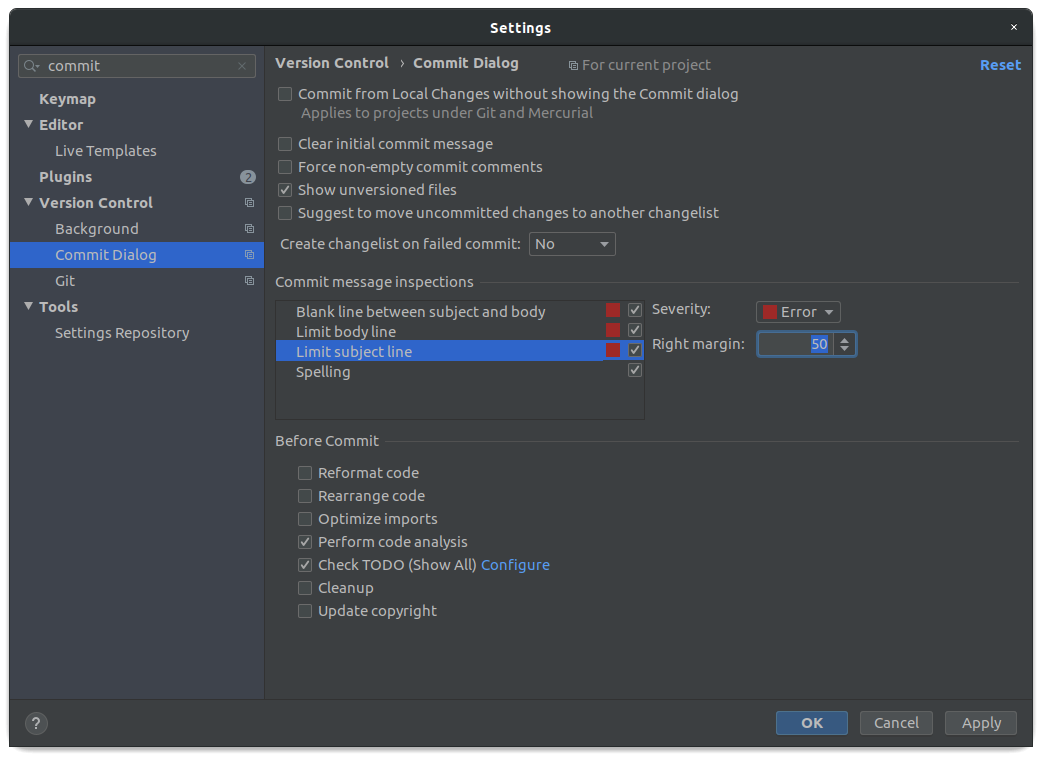
\includegraphics[scale=0.25]{images/jetbrains-commit-message-settings.png}
      \caption{JetBrain's IDEs commit message settings}
      \label{fig:commit-settings}
  \end{figure}

\end{frame}

\begin{frame}[fragile]
  \frametitle{Commit Message Line Limits + Jetbrains}
  
  \begin{figure}
      \centering
      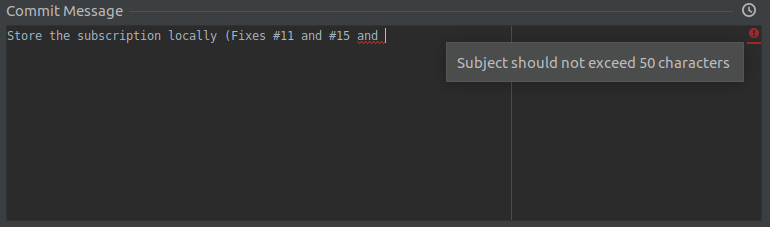
\includegraphics[scale=0.35]{images/jetbrains-commit-message.png}
      \caption{JetBrain's IDEs commit message dialog}
      \label{fig:commit-dialog}
  \end{figure}

\end{frame}


\plain{}{Questions?}

\end{document}
